\documentclass[12pt]{article}
%\usepackage[portuguese]{babel}
\usepackage[utf8]{inputenc}
\usepackage[usenames,dvipsnames]{color}
\usepackage{setspace}
\usepackage{amsmath}
\usepackage{amsfonts}
\usepackage{amssymb}
\usepackage{mathtools}
\usepackage[top=3cm, bottom=2cm, left=3cm, right=2cm]{geometry}
\usepackage{tikz}
\usepackage{indentfirst}
\usepackage{algorithm} % algorithms
\usepackage{algpseudocode} % algorithms
\usepackage{textcomp}
\title{Relatorio IC}

% packages added by Marcelo
%
\usepackage{lscape}    % for landscape pages
\usepackage{hyperref}  % to allow hyperlinks
\usepackage{booktabs}  % nicer table borders
\usepackage{subfigure} % add subfigures

\graphicspath{{./figures/}} 

\definecolor{myblue}{RGB}{80,80,160}
\definecolor{mygreen}{RGB}{80,160,80}
\setstretch{1.5}

\begin{document}

\begin{center}
{\Large Stochastic U-Curve Branch and Bound \\}
\bigskip
{\bf Student:} \href{mailto:estrela.gustavo.matos@gmail.com}{Gustavo Estrela de Matos} \\
        {\bf Advisor:} \href{mailto:ulisses@ece.tamu.edu}{Dr. Ulisses Braga-Neto}
\end{center}

\section{Input Generation}
To generate the input for the problem we created two functions. The first creates a vector of floating points that simulates the values of a chain of a boolean lattice that respects the U-Curve assumption; and the second one adds a random noise to the values of the vector.

\subsection{Chain Generation}
The algorithm receives three parameters: $n$, $max\_distance$ and $center$; and returns as output a vector that has values from $0$ to $1$ and respects the U-Curve assumption. The first parameter defines the size of the chain; the second represents the greatest possible difference between the values of neighbour nodes, which is a random value uniformily distributed between $0$ and $max\_distance$; and the last represents the index of the node with minimum value.

\begin{algorithm}[t]
\caption{U-Curve Input Creator}
\begin{algorithmic}[1]
\Procedure{GeneratePoints}{$n, max\_distance, center$}
    \State $points \gets \{0, ..., 0\}$
    \State $minimum \gets \frac{random ()}{2}$
    \State $points[center] \gets minimum$
    \State
    \For {$i \in \{0, ..., center - 1\}$}
        \State $points[i] \gets points[i + 1] + (1 - points[i + 1]) * random ()$
    \EndFor
    \For {$i \in \{center + 1, ..., n - 1\}$}
        \State $points[i] \gets points[i - 1] + (1 - points[i - 1]) * random ()$
    \EndFor
    \State
    \State $j \gets n * random ()$
    \State $plain_size \gets (n - j) * random ()$
    \For {$k \in \{1, ..., plain_size\}$} \Comment Creates a plain area in the chain
        \State $points[j + k] \gets points[j]$
    \EndFor
    \Return $points$
\EndProcedure
\end{algorithmic}
\end{algorithm}

\subsection{Noise}
The noise is applied to the vector created by $GeneratePoints$, by adding a value uniformily distributed in the interval 
$[-\alpha \frac{curve\_amplitude}{n}, \alpha \frac{curve\_amplitude}{n}]$, where $curve\_amplitude = max(v) - min (v)$ and $\alpha$ is a noise parameter.

\begin{figure}[H]
\caption{Example of a curve generated with $\alpha = 0$}
\centering
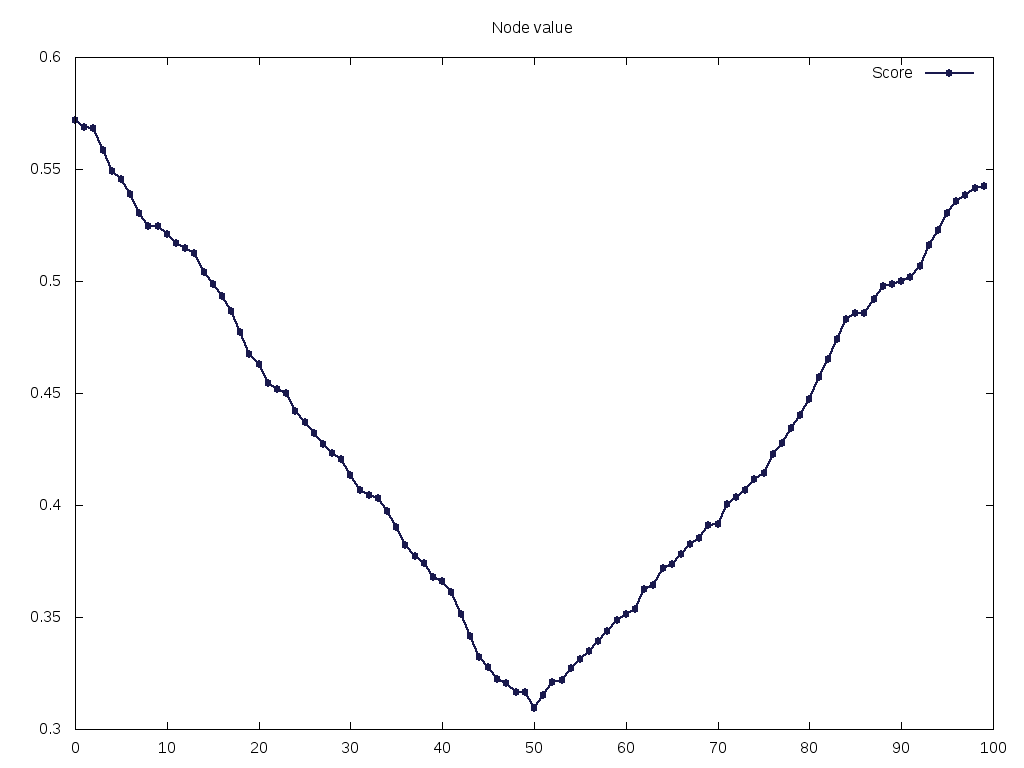
\includegraphics[scale=.5]{alpha_zero_curve}
\end{figure}

\begin{figure}[H]
\caption{Example of a curve generated with $\alpha = 1$}
\centering
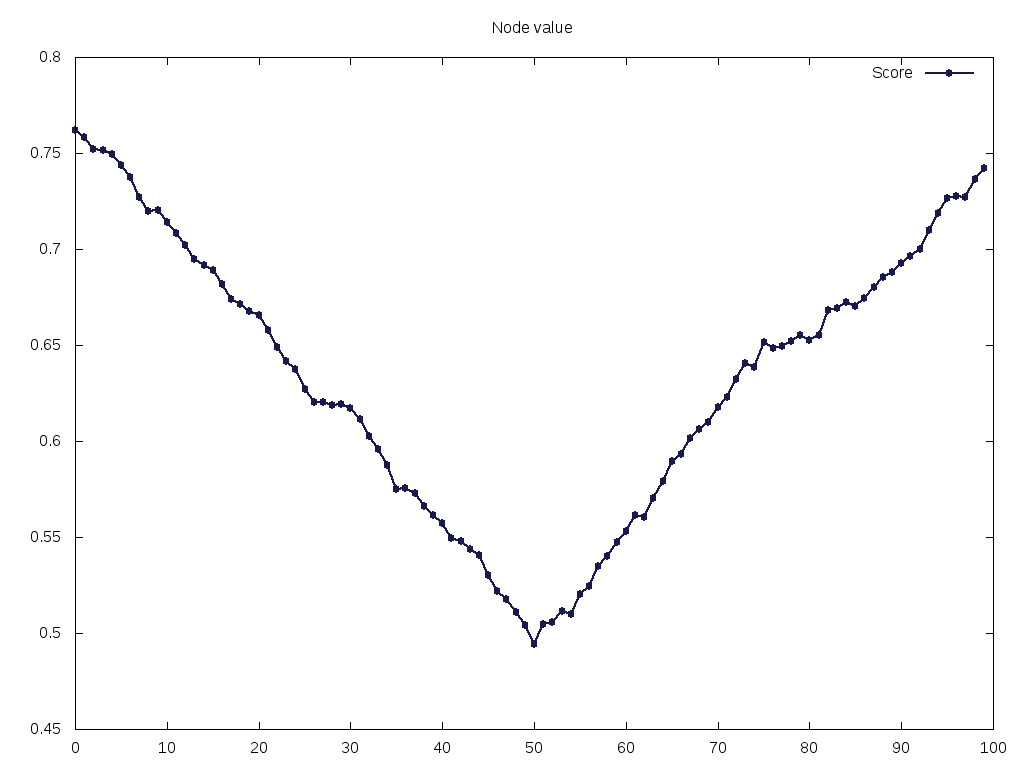
\includegraphics[scale=.5]{alpha_one_curve}
\end{figure}

\begin{figure}[H]
\caption{Example of a curve generated with $\alpha = 2$}
\centering
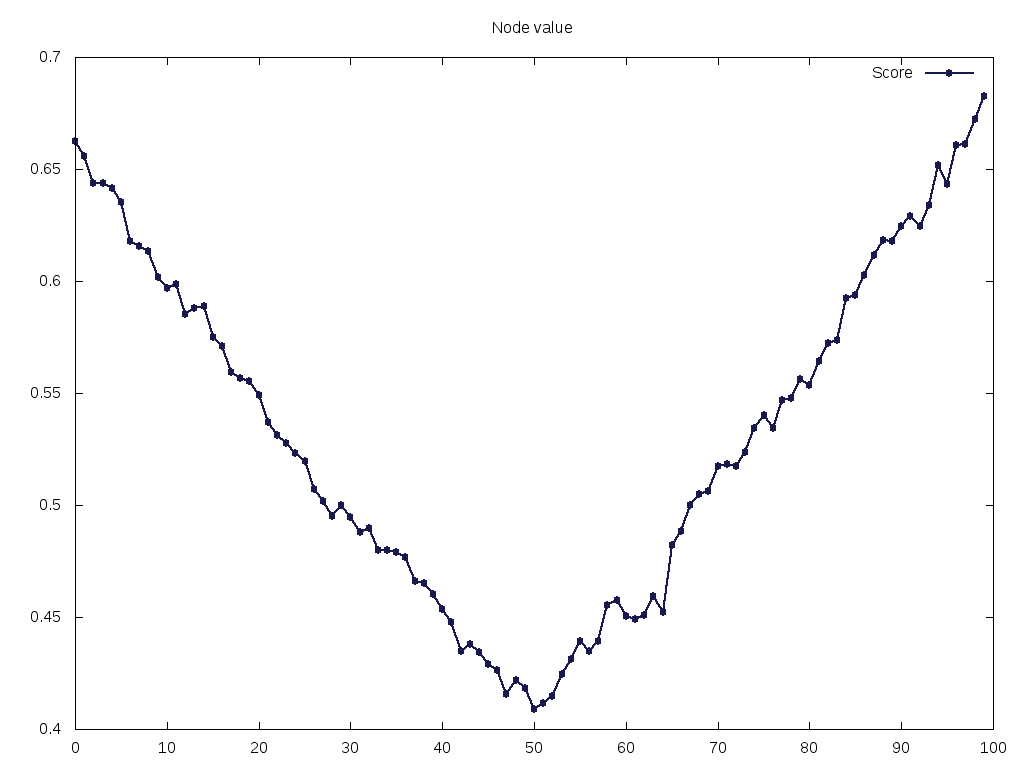
\includegraphics[scale=.5]{alpha_two_curve}
\end{figure}

\newpage
\section{Bisection Algorithms}
\subsection{Traditional Bisection}
This is the simplest bisection algorithm we implemented. The basic idea of this algorithm is to divide the original problem in two halfs and, by analysing the neighbours of the node in the middle, determine which half has the minimum and then solve this half recursively. To guarantee the optimally of the algorithm (when the input respects the U-Curve assumption) we solve both halfs when the neighbours can't determine if the minimum lies to the left or right of the middle point.
\begin{algorithm}[h]
\caption{}
\begin{algorithmic}[1]
\Procedure{Bisection}{$v$}
    \State $n \gets v.length$
    \State $i \gets n / 2$
    \If {$(valley (v, i))$}
        \State
        \Return $v[i]$
    \Else
        \State $direction \gets SelectSide (v, i)$
        \If {$direction = Left$}
            \State
            \Return $Bisection ([v_i, ..., v_n])$
        \ElsIf {$direction = Right$}
            \State
            \Return $Bisection ([v_0, ..., v_{i - 1}])$
        \Else \Comment Unknown direction
            \State
            \Return $min (Bisection ([v_0, ..., v_{i - 1}]), Bisection ([v_i, ..., v_n]))$
        \EndIf
    \EndIf

\EndProcedure
\end{algorithmic}
\end{algorithm}

\begin{algorithm}[h]
\caption{}
\begin{algorithmic}[1]
\Procedure{SelectSide}{$v, i$}
    \State $d = v[i + 1] - v[i - 1]$
    \If {$|d| < \epsilon$}
        \State
        \Return Unknown
    \ElsIf {$d > 0$}
        \State
        \Return Left
    \Else
        \State
        \Return Right
    \EndIf
\EndProcedure
\end{algorithmic}
\end{algorithm}

\subsection {Mid-neighbour Bisection}
As an attempt to minimize the effects of noise in the traditional bisection algorithm we developed the Mid-neighbour Bisection, which brings two new ideas to the traditional bisection, that changes the evaluated points and also how we divide the problem in smaller problems.

The first idea consists in changing the points that are evaluated to decide which side to go. Instead of looking to the neighbours of the middle point, we now evaluate the points that are in the middle of the left half and right half. After evaluating these points, we calculate the difference between the left-middle point and middle point and also the difference between the right-middle point and the middle point to get two abstract slopes that can guarantee us which fraction of the input has the minimum value. 

The second idea considers the "reliabillity" of the abstract slopes mentioned before, for instance, if we say that the left slope (middle point - left-middle point) is negative, it's more likely that the function is going to increase from the left-middle point and before if the distance between these two points is greater. That happens because if the function decreases from the left-middle point and before, then the left-middle point suffered some noise that caused a peak (an inverted u-shape) and, considering that the points should describe a u-shape that would imply in a bigger noise for bigger distances of middle point and lef-middle point. We modeled the "reliability" of the abstract slope as a linear function that decreases from one to zero in $lg n$ steps.

The abstracts slopes are reduced to three different cases: 1 for growing, -1 for decreasing and 0 for plain areas or unreliable difference. Since we have two different slopes

\end{document}

